\documentclass{article}
\nonstopmode

% Packages
% 
\usepackage{amsfonts,amssymb,amsmath}
\usepackage{tikz}
\usetikzlibrary{automata,positioning,arrows}
\usepackage[margin=1in]{geometry}

% Common Declarations
% 
% Make sure you change the author in common.tex
% 

\author{Michael Rettus}
\def\term{Winter 2021}
\def\course{CSCI~301}

% 
%
\setlength{\parskip}{1em}
\setlength{\parindent}{0in}

%
%
\newcounter{thequestion}
\newcommand{\question}{%
  \stepcounter{thequestion}%
  \noindent%
  \textbf{\arabic{thequestion}\quad}%
}
\newcommand{\answer}{%
  \par\noindent%
  \textbf{Answer\\}%
}



% Local Declarations
% 
\title{\course, \term\\Math Exercises \#4}
\tikzset{
  ->, >=stealth', node distance=.75in, initial text=$$,
  every state/.style={thick, fill=gray!10}
  }

% The document
% 
\begin{document}
\maketitle

\question%
The set of all strings that have exactly one doubled digit in them.  In other
words, either 11 or 00 occurs in the string, but not both, and it only occurs
once.
\begin{center}
  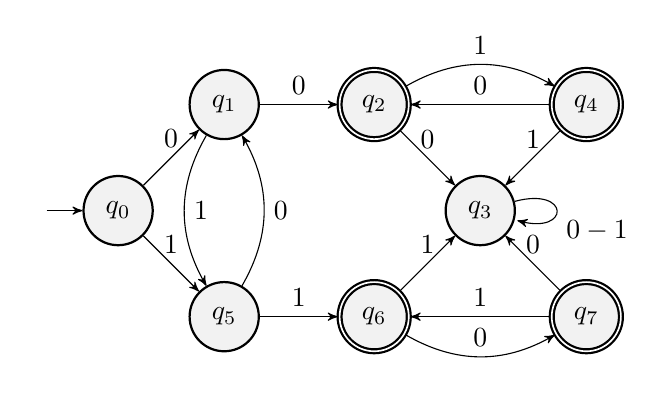
\begin{tikzpicture}

    \node [state, initial] at (1,1) (q0) {$q_0$};

    \node [state, above right of=q0] (q1) {$q_1$};    
    \node [state, accepting, right of=q1] (q2) {$q_2$};
    \node [state, below right of=q2] (q3) {$q_3$};
    \node [state, accepting, above right of=q3] (q4) {$q_4$};
    \node [state, below right of=q0] (q5) {$q_5$};
    \node [state, accepting, right of=q5] (q6) {$q_6$};
    \node [state, accepting, below right of=q3] (q7) {$q_7$};
    % This is an edge from q0 to q1 with the label $0-1$ above the edge.  
    \draw (q0) edge[above] node{$0$} (q1);
    \draw (q0) edge[above] node{$1$} (q5);
    \draw (q1) edge[right, bend right] node{$1$} (q5);
    \draw (q5) edge[right, bend right] node{$0$} (q1);
    \draw (q1) edge[above] node{$0$} (q2);
    \draw (q2) edge[above] node{$0$} (q3);
    \draw (q2) edge[above, bend left] node{$1$} (q4);
    \draw (q4) edge[above] node{$0$} (q2);
    \draw (q4) edge[above] node{$1$} (q3);
    \draw (q5) edge[above] node{$1$} (q6);
    \draw (q6) edge[above] node{$1$} (q3);
    \draw (q6) edge[above, bend right] node{$0$} (q7);
    \draw (q7) edge[above] node{$1$} (q6);
    \draw (q7) edge[above] node{$0$} (q3);
    % This is an edge from q1 to q1 looping below the state
    % with the label $0-1$ below and right of the edge.
    \draw (q3) edge[loop right, below right] node{$0-1$} (q3);
  \end{tikzpicture}
\end{center}
\answer This DFA is pretty symmetric since top and bottom do essentially the same thing 
except top finds doubled 00's and the other doubled 11's. I took the route of excluding 
triples considering them two doubles. Q1,2,4 are compliments of Q5,6,7 respectively. From initial 0 changes state to q1, and 1 to q5 where they will swap states between 1 and 5 until a double comes in. double 00 = state of q2 and double 11 is state of q6. These are accepting states so if it terminates there we're good. from there a third 0 or 1 changes the state to q3 and traps the string. Changing the digit however changes the state to q4 or q7 respectively and continue to swap between 2and 4 or 6 and 7 as long as there are no further doubles. Double 0s then q2 and q7 change state to q3, while q6 and q4 do the same for double 1s. Again q3 is a trap so any set of second doubles and the string is reject. As long as there is only one set of doubles the string will be accepted in one of the 4 final states.\\

\pagebreak
\question%
The set of all strings beginning with a 1 such that, interpreted as a binary
representation of an integer, it has a remainder of 1 when divided by 3.  For
example, the binary number $1010_b$ is decimal $10$.  When you divide 10 by 3
you get a remainder of 1, so $1010$ is in the language.  However, the binary
number $1111_b$ is decimal $15$.  When you divide 15 by 3 you get a remainder of
0, so $1111$ is not in the language.

\begin{center}
  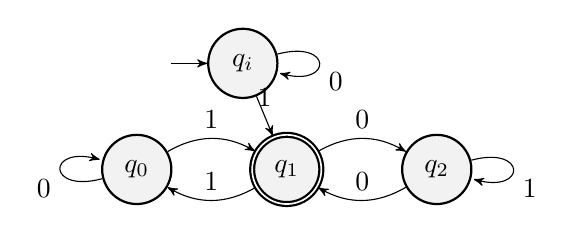
\begin{tikzpicture}

    \node [state, initial] at (1,1) (qi) {$q_i$};
    \node [state, below left of =qi]  (q0) {$q_0$};
    \node [state, accepting, right of=q0] (q1) {$q_1$};    
    \node [state, right of=q1] (q2) {$q_2$};
    \draw (qi) edge[loop right, below right] node{$0$} (qi);
    \draw (qi) edge[above] node{$1$} (q1);
    \draw (q0) edge[loop left, below left] node{$0$} (q0);
    \draw (q0) edge[above, bend left] node{$1$} (q1);
    \draw (q1) edge[above, bend left] node{$0$} (q2);
    \draw (q2) edge[loop right, below right] node{$1$} (q2);
    \draw (q2) edge[above, bend left] node{$0$} (q1);
    \draw (q1) edge[above, bend left] node{$1$} (q0);

 \end{tikzpicture}
\end{center}
\answer
qi is the initial state and used to bleed off 0's preceding the initial 1
q0 = remainder 0, q1=remainder 1, q2 is remainder2 0/3 =0 so 0 loops to itself in q0, 1/3=1 so 1 in q0 goes to q1, from q1 ,2/3=2 so 0 in q1 loops to q2, 3/3=0so 1 in q1 loops to q0, in q2 4/3=1 so 0 loops to q1, and 5/3=2 so 1 loops back into q2 from there every other binary combination will work
\end{document}
